\documentclass[10pt,compress]{beamer}
%\documentclass[fleqn,xcolor=dvipsnames]{beamer}
% \usetheme{Madrid}
% \usetheme{Boadilla}
% \usetheme{default}
% \usetheme{Warsaw}
% \usetheme{CambridgeUS}
% \usetheme{Sybila}
\usetheme[hideothersubsections]{Berkeley}
% \usetheme[hideothersubsections]{PaloAlto}
%%\usetheme[hideothersubsections]{Goettingen}
%\usetheme{CambridgeUS}
% \usetheme{Bergen} % This template has nagivation on the left
% \usetheme{Frankfurt} % Similar to the default with an extra region at the top.

% Uncomment the following line if you want page numbers and use Warsaw theme%
%\setbeamertemplate{footline}[page number]

\definecolor{aggiemaroon}{RGB}{80,0,0} % Official RGB code for aggie maroon
\usecolortheme[named=aggiemaroon]{structure}
\useoutertheme{shadow}
\useinnertheme{rounded}
\setbeamertemplate{navigation symbols}{}
\setbeamerfont{structure}{family=\rmfamily,series=\bfseries}
\usefonttheme[stillsansseriftext]{serif}

\usepackage{algorithm}
\usepackage{algpseudocode}
\usepackage{amsmath}
\usepackage{caption}
\usepackage{graphicx,comment}
\usepackage[english]{babel}
\usepackage{graphicx}
\usepackage{rotating}
\usepackage{multicol}
\usepackage{hyperref}
\usepackage{enumerate}
\usepackage{tikz}
\usepackage{graphicx}
\usepackage{bm}
\usepackage{theoremref}
\usepackage{colortbl}

\usebackgroundtemplate{
\tikz\node[opacity=0.025, rotate = 0] {\includegraphics[height=\paperheight,width=\paperwidth]{TAM-Logo.png}};}
%{\includegraphics[height=1in,width=1in]{TAM-Logo.png}};}

\title[Texas A\&M University]{Binary Heaps}

\author [Barbieri]{Dante Barbieri}

\date[ 11/19/2021]{November 19, 2021}

\institute[Texas A\&M U.] % (optional, but mostly needed)
{\emph{Data Structures and Algorithms}, Texas A\&M University, College Station, TX \\
 \includegraphics[scale=0.60]{TAM-Logo1.png} \\ [0.0 cm]
 }



\AtBeginSection[]
{
  \begin{frame}<beamer>
    \frametitle{Section \thesection}
    \tableofcontents[currentsection,currentsubsection]
  \end{frame}
}

\usetikzlibrary{automata, positioning, arrows, matrix, positioning}

\tikzset{
-, % makes the edges undirected
>=stealth', % makes the arrow heads bold
node distance=2cm, % specifies the minimum distance between two nodes. Change if necessary.
every state/.style={thick, white, draw=black, fill=aggiemaroon}, % sets the properties for each ’state’ node
initial text=$ $, % sets the text that appears on the start arrow
}

\tikzset{
  selected/.append style={state, black, draw=black, fill=white}
}

\tikzset{ 
table/.style={
  matrix of nodes,
  row sep=-\pgflinewidth,
  column sep=-\pgflinewidth,
  nodes={draw=black,text width=3.75ex,align=center},
  text depth=0.25ex,
  text height=1.8ex,
  nodes in empty cells
  },
texto/.style={font=\footnotesize\sffamily},
title/.style={font=\small\sffamily}
}

\begin{document}

\begin{frame}
  \titlepage
\end{frame}

%\begin{frame}
%\frametitle{Overview} 
%\tableofcontents
%\end{frame}

\section{Data Structure}

\begin{frame}
  \frametitle{Binary Heap Conceptually}
  \begin{flushleft}
    \begin{figure}[ht] % ’ht’ tells LaTeX to place the figure ’here’ or at the top of the page
      \centering % centers the figure
      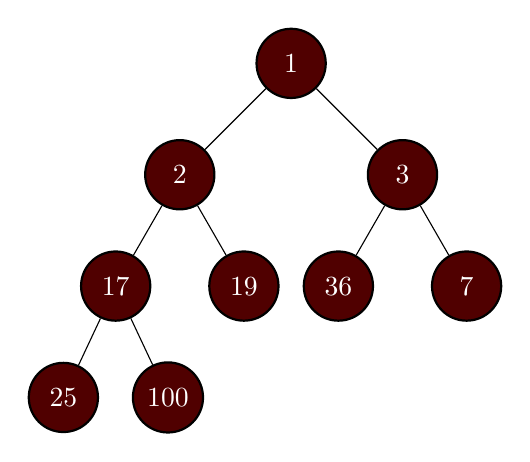
\begin{tikzpicture}
        \node[state] (1) {1};
        \node[state, below left of=1] (2) {2};
        \node[state, below right of=1] (3) {3};
        \node[state, below left of=2, xshift=0.6cm] (17) {17};
        \node[state, below right of=2, xshift=-0.6cm] (19) {19};
        \node[state, below left of=3, xshift=0.6cm] (36) {36};
        \node[state, below right of=3, xshift=-0.6cm] (7) {7};
        \node[state, below left of=17, xshift=0.75cm] (25) {25};
        \node[state, below right of=17, xshift=-0.75cm] (100) {100};

        \draw (1) edge node{} (2)
        (1) edge node{} (3)
        (2) edge node{} (17)
        (2) edge node{} (19)
        (3) edge node{} (36)
        (3) edge node{} (7)
        (17) edge node{} (25)
        (17) edge node{} (100);
      \end{tikzpicture}
      \caption{Tree Representation of a Binary Min-Heap}
      \label{fig:tree_bin_min_heap}
    \end{figure}
  \end{flushleft}
\end{frame}

\newtheorem*{complete_binary_tree_property}{Complete Binary Tree Property}

\subsection{Structural Property}

\begin{frame}{Binary Heap Structural Property}
  \begin{itemize}
    \item The structure of a Binary Heap is a particular form of a Binary Tree.
  \end{itemize}
  \begin{complete_binary_tree_property}
    A heap $T$ with height $h$ is a \textbf{complete} binary tree, that is, levels $0$,$1$,$2$,$\ldots$,$h-1$ of $T$ have the maximum number of nodes possible (namely, level $i$ has $2^i$ nodes, for \(0\leq 1\leq h-1\)) and the nodes at level $h$ fill this level from left to right.
  \end{complete_binary_tree_property}
  \begin{itemize}
    \item All Binary Heaps must always follow the Complete Binary Tree Property.
  \end{itemize}

  The above definition comes from \textit{Data Structures \& Algorithms} by Goodrich et al.
\end{frame}

\subsubsection{Array Representation}
\begin{frame}
  \frametitle{Preferred Method to Store Binary Heaps}
  We take advantage of the Structural Property in order to store the Binary Heap in an Array.
  \begin{flushleft}
    \begin{figure}[ht] % ’ht’ tells LaTeX to place the figure ’here’ or at the top of the page
      \centering % centers the figure
      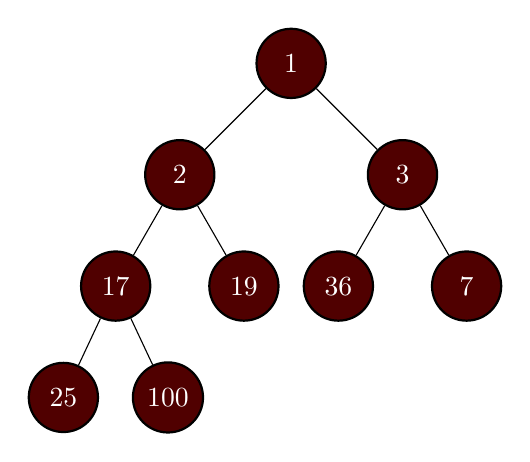
\begin{tikzpicture}
        \node[state] (1) {1};
        \node[state, below left of=1] (2) {2};
        \node[state, below right of=1] (3) {3};
        \node[state, below left of=2, xshift=0.6cm] (17) {17};
        \node[state, below right of=2, xshift=-0.6cm] (19) {19};
        \node[state, below left of=3, xshift=0.6cm] (36) {36};
        \node[state, below right of=3, xshift=-0.6cm] (7) {7};
        \node[state, below left of=17, xshift=0.75cm] (25) {25};
        \node[state, below right of=17, xshift=-0.75cm] (100) {100};

        \draw (1) edge node{} (2)
        (1) edge node{} (3)
        (2) edge node{} (17)
        (2) edge node{} (19)
        (3) edge node{} (36)
        (3) edge node{} (7)
        (17) edge node{} (25)
        (17) edge node{} (100);
      \end{tikzpicture}
      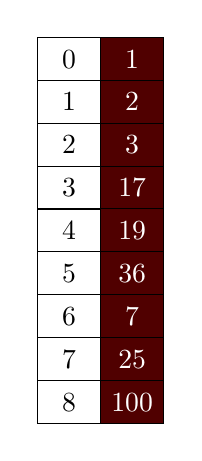
\begin{tikzpicture}[ampersand replacement=\&, node distance =0pt and 0.5cm]
        \matrix[table]
        {
        0 \& |[white, fill=aggiemaroon, draw=black]| 1 \\
        1 \& |[white, fill=aggiemaroon, draw=black]| 2 \\
        2 \& |[white, fill=aggiemaroon, draw=black]| 3 \\
        3 \& |[white, fill=aggiemaroon, draw=black]| 17 \\
        4 \& |[white, fill=aggiemaroon, draw=black]| 19 \\
        5 \& |[white, fill=aggiemaroon, draw=black]| 36 \\
        6 \& |[white, fill=aggiemaroon, draw=black]| 7 \\
        7 \& |[white, fill=aggiemaroon, draw=black]| 25 \\
        8 \& |[white, fill=aggiemaroon, draw=black]| 100 \\
        };
      \end{tikzpicture}
      \caption{Array Representation of the Binary Min-Heap from Concept}
      \label{fig:array_rep}
    \end{figure}
  \end{flushleft}
\end{frame}

\begin{frame}
  \frametitle{Specifics of Array Representation}
  \begin{tabular}{c|c|c|c|c|c|c|c|c|c|}\cline{2-10}
    Array Index & 0                                           & 1                                           & 2                                           & 3                                            & 4                                            & 5                                            & 6                                           & 7                                            & 8                                             \\\hline
    Heap Value  & \cellcolor{aggiemaroon}\textcolor{white}{1} & \cellcolor{aggiemaroon}\textcolor{white}{2} & \cellcolor{aggiemaroon}\textcolor{white}{3} & \cellcolor{aggiemaroon}\textcolor{white}{17} & \cellcolor{aggiemaroon}\textcolor{white}{19} & \cellcolor{aggiemaroon}\textcolor{white}{36} & \cellcolor{aggiemaroon}\textcolor{white}{7} & \cellcolor{aggiemaroon}\textcolor{white}{25} & \cellcolor{aggiemaroon}\textcolor{white}{100} \\\cline{2-10}
  \end{tabular}
  \begin{align*}
    \text{Parent Index}      & = \left\lfloor\frac{\text{Index} - 1}{2}\right\rfloor      \\
    \text{Left Child Index}  & = 2\times\text{Index} + 1                                  \\
    \text{Right Child Index} & = 2\times\text{Index} + 2 = 2\left(\text{Index} + 1\right)
  \end{align*}
  \[
    n = \text{Array Length}
  \]
  \[
    h = \left\lfloor\log_2 n\right\rfloor
  \]
  \[
    \text{Root Index} = 0
  \]
  \[
    \text{Leaf Index} \Rightarrow \text{Left Child Index} \geq n
  \]
  Remember: \texttt{vector} is a good way to use Arrays that grow in C++.
\end{frame}

\newtheorem*{bst_ordering}{Recall -- Binary Search Tree Order Property}
\newtheorem*{min_heap_ordering}{Min-Heap Order Property}
\newtheorem*{max_heap_ordering}{Max-Heap Order Property}

\subsection{Ordering Property}

\begin{frame}{Binary Heap Ordering}
  \begin{itemize}
    \item The second qualification to be considered a Binary Heap is the satisfaction of an ordering property that organizes the locations of nodes in a heap relative to one another.
    \item This is similar to the Binary Search Tree ordering property.
  \end{itemize}
  \begin{bst_ordering}
    In a binary search tree $T$, for every node $v$ other than the leaves (external nodes), the following are true:
    \begin{enumerate}
      \item the value associated with $v$ is greater than or equal to the value associated with $v$'s left child,
      \item the value associated with $v$ is less than or equal to the value associated with $v$'s right child, and
      \item any values equivalent to the value associated with $v$ lie either entirely in the left subtree of $v$ or entirely in the right subtree of $v$ for all $v$ with minimum depth in $T$.
    \end{enumerate}
  \end{bst_ordering}
\end{frame}

\begin{frame}{Binary Min-Heap Ordering}
  \begin{itemize}
    \item The ``key'' in the below definition is the value compared between two nodes to determine their order.
    \item This is similar to the practice for a Binary Search Tree, but allows us to compare only parts of an object.\\
          e.g.
          \begin{itemize}
            \item Compare a students's GPA but not their name
            \item Compare a CPU job's priority but not its length or its ID
          \end{itemize}
  \end{itemize}
  \begin{min_heap_ordering} \thlabel{min_order}
    In a heap $T$, for every node $v$ other than the root, the key associated with $v$ is greater than or equal to the key associated with $v$'s parent.
  \end{min_heap_ordering}

  The above definition comes from \textit{Data Structures \& Algorithms} by Goodrich et al.
\end{frame}

\begin{frame}{Binary Max-Heap Ordering}
  \begin{itemize}
    \item This is identical to the Min-Heap Order Property, except the comparison goes the other direction.
  \end{itemize}
  \begin{max_heap_ordering}
    In a heap $T$, for every node $v$ other than the root, the key associated with $v$ is less than or equal to the key associated with $v$'s parent.
  \end{max_heap_ordering}

  The above definition comes from \textit{Data Structures \& Algorithms} by Goodrich et al.
\end{frame}

\section{Operations}

\subsection{Insert}

\begin{frame}{Insertion}
  First we need to ensure that the structural property of the Heap is maintained.
  \begin{figure}[ht] % ’ht’ tells LaTeX to place the figure ’here’ or at the top of the page
    \centering % centers the figure
    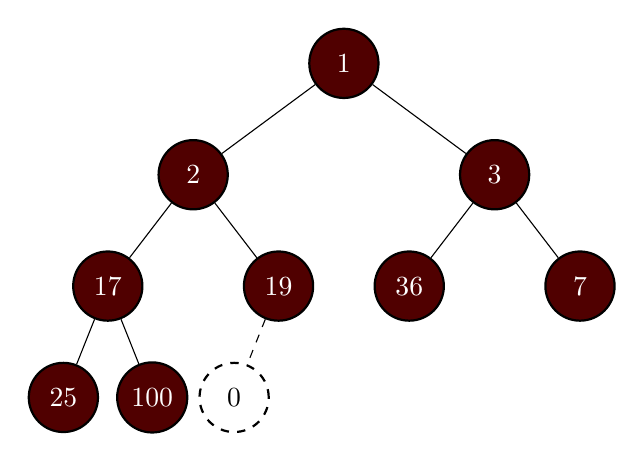
\begin{tikzpicture}
      \node[state] (1) {1};
      \node[state, below left of=1, xshift=-0.5cm] (2) {2};
      \node[state, below right of=1, xshift=0.5cm] (3) {3};
      \node[state, below left of=2, xshift=0.33cm] (17) {17};
      \node[state, below right of=2, xshift=-0.33cm] (19) {19};
      \node[state, below left of=3, xshift=0.33cm] (36) {36};
      \node[state, below right of=3, xshift=-0.33cm] (7) {7};
      \node[state, below left of=17, xshift=0.85cm] (25) {25};
      \node[state, below right of=17, xshift=-0.85cm] (100) {100};
      \node[selected, dashed, below left of=19, xshift=0.85cm] (0) {0};

      \draw (1) edge node{} (2)
      (1) edge node{} (3)
      (2) edge node{} (17)
      (2) edge node{} (19)
      (3) edge node{} (36)
      (3) edge node{} (7)
      (17) edge node{} (25)
      (17) edge node{} (100)
      (19) edge[dashed] node{} (0);
    \end{tikzpicture}
    \caption{Insert `0' to the Binary Heap from before}
    \label{fig:bin_min_heap_insert_structure}
  \end{figure}
\end{frame}

\subsubsection{Upheap}

\begin{frame}{Upheap}
  Once `0' is inserted structurally, we need to fix the ordering. One way to do this is to continue up the heap until the order is correct or the new node becomes the root. This process is called Upheap.
  \begin{figure}[ht] % ’ht’ tells LaTeX to place the figure ’here’ or at the top of the page
    \centering % centers the figure
    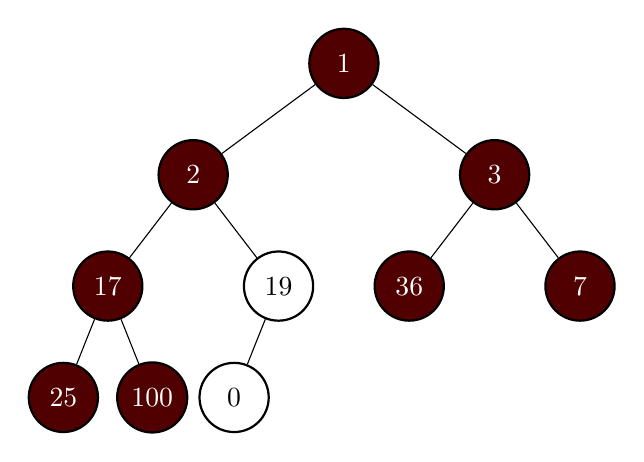
\begin{tikzpicture}
      \node[state] (1) {1};
      \node[state, below left of=1, xshift=-0.5cm] (2) {2};
      \node[state, below right of=1, xshift=0.5cm] (3) {3};
      \node[state, below left of=2, xshift=0.33cm] (17) {17};
      \node[selected, below right of=2, xshift=-0.33cm] (19) {19};
      \node[state, below left of=3, xshift=0.33cm] (36) {36};
      \node[state, below right of=3, xshift=-0.33cm] (7) {7};
      \node[state, below left of=17, xshift=0.85cm] (25) {25};
      \node[state, below right of=17, xshift=-0.85cm] (100) {100};
      \node[selected, below left of=19, xshift=0.85cm] (0) {0};

      \draw (1) edge node{} (2)
      (1) edge node{} (3)
      (2) edge node{} (17)
      (2) edge node{} (19)
      (3) edge node{} (36)
      (3) edge node{} (7)
      (17) edge node{} (25)
      (17) edge node{} (100)
      (19) edge node{} (0);
    \end{tikzpicture}
    \caption{Compare `19' and `0'}
    \label{fig:comp_19_0}
  \end{figure}
\end{frame}

\begin{frame}{Upheap}
  We swapped `0' and `19' because they were out of order. Now we continue up the tree.
  \begin{figure}[ht] % ’ht’ tells LaTeX to place the figure ’here’ or at the top of the page
    \centering % centers the figure
    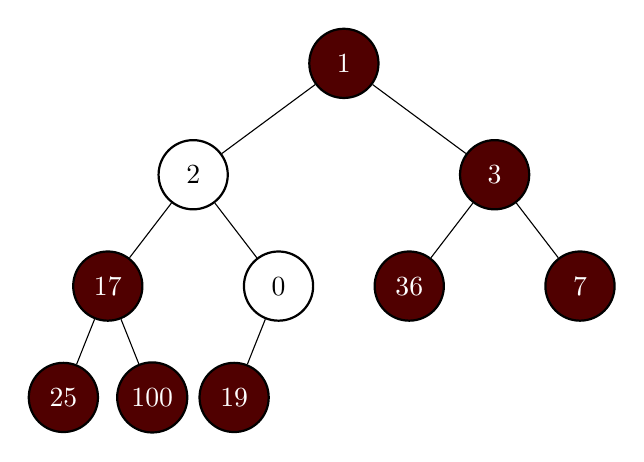
\begin{tikzpicture}
      \node[state] (1) {1};
      \node[selected, below left of=1, xshift=-0.5cm] (2) {2};
      \node[state, below right of=1, xshift=0.5cm] (3) {3};
      \node[state, below left of=2, xshift=0.33cm] (17) {17};
      \node[selected, below right of=2, xshift=-0.33cm] (0) {0};
      \node[state, below left of=3, xshift=0.33cm] (36) {36};
      \node[state, below right of=3, xshift=-0.33cm] (7) {7};
      \node[state, below left of=17, xshift=0.85cm] (25) {25};
      \node[state, below right of=17, xshift=-0.85cm] (100) {100};
      \node[state, below left of=0, xshift=0.85cm] (19) {19};

      \draw (1) edge node{} (2)
      (1) edge node{} (3)
      (2) edge node{} (17)
      (2) edge node{} (0)
      (3) edge node{} (36)
      (3) edge node{} (7)
      (17) edge node{} (25)
      (17) edge node{} (100)
      (0) edge node{} (19);
    \end{tikzpicture}
    \caption{Compare `2' and `0'}
    \label{fig:comp_2_0}
  \end{figure}
\end{frame}

\begin{frame}{Upheap}
  \begin{figure}[ht] % ’ht’ tells LaTeX to place the figure ’here’ or at the top of the page
    \centering % centers the figure
    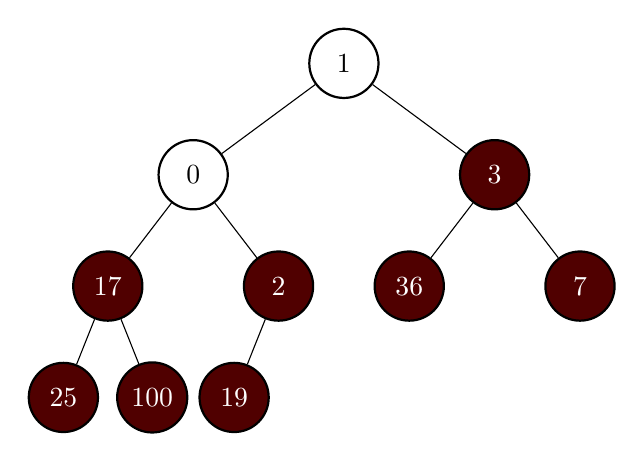
\begin{tikzpicture}
      \node[selected] (1) {1};
      \node[selected, below left of=1, xshift=-0.5cm] (0) {0};
      \node[state, below right of=1, xshift=0.5cm] (3) {3};
      \node[state, below left of=0, xshift=0.33cm] (17) {17};
      \node[state, below right of=0, xshift=-0.33cm] (2) {2};
      \node[state, below left of=3, xshift=0.33cm] (36) {36};
      \node[state, below right of=3, xshift=-0.33cm] (7) {7};
      \node[state, below left of=17, xshift=0.85cm] (25) {25};
      \node[state, below right of=17, xshift=-0.85cm] (100) {100};
      \node[state, below left of=2, xshift=0.85cm] (19) {19};

      \draw (1) edge node{} (0)
      (1) edge node{} (3)
      (0) edge node{} (17)
      (0) edge node{} (2)
      (3) edge node{} (36)
      (3) edge node{} (7)
      (17) edge node{} (25)
      (17) edge node{} (100)
      (2) edge node{} (19);
    \end{tikzpicture}
    \caption{Compare `2' and `0'}
    \label{fig:comp_1_0}
  \end{figure}
\end{frame}

\begin{frame}{Upheap}
  We stop here because our node has become the root.
  \begin{figure}[ht] % ’ht’ tells LaTeX to place the figure ’here’ or at the top of the page
    \centering % centers the figure
    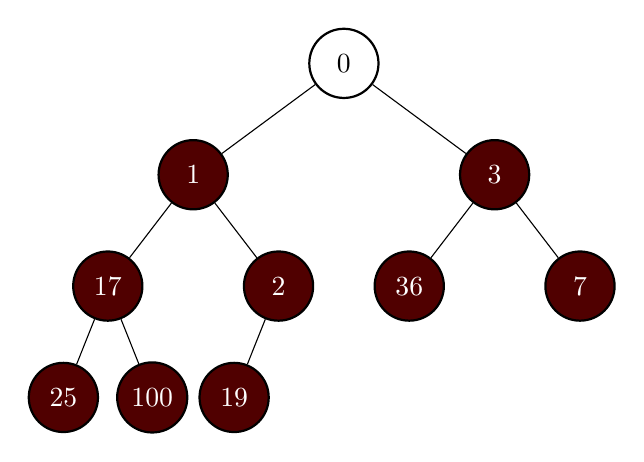
\begin{tikzpicture}
      \node[selected] (0) {0};
      \node[state, below left of=0, xshift=-0.5cm] (1) {1};
      \node[state, below right of=0, xshift=0.5cm] (3) {3};
      \node[state, below left of=1, xshift=0.33cm] (17) {17};
      \node[state, below right of=1, xshift=-0.33cm] (2) {2};
      \node[state, below left of=3, xshift=0.33cm] (36) {36};
      \node[state, below right of=3, xshift=-0.33cm] (7) {7};
      \node[state, below left of=17, xshift=0.85cm] (25) {25};
      \node[state, below right of=17, xshift=-0.85cm] (100) {100};
      \node[state, below left of=2, xshift=0.85cm] (19) {19};

      \draw (0) edge node{} (1)
      (0) edge node{} (3)
      (1) edge node{} (17)
      (1) edge node{} (2)
      (3) edge node{} (36)
      (3) edge node{} (7)
      (17) edge node{} (25)
      (17) edge node{} (100)
      (2) edge node{} (19);
    \end{tikzpicture}
    \caption{Base case as `0' is the new root}
    \label{fig:base_case}
  \end{figure}
\end{frame}

\begin{frame}{Upheap}
  \begin{figure}[ht] % ’ht’ tells LaTeX to place the figure ’here’ or at the top of the page
    \centering % centers the figure
    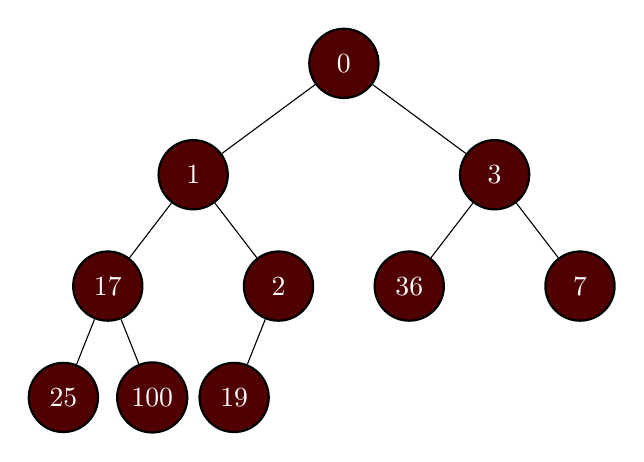
\begin{tikzpicture}
      \node[state] (0) {0};
      \node[state, below left of=0, xshift=-0.5cm] (1) {1};
      \node[state, below right of=0, xshift=0.5cm] (3) {3};
      \node[state, below left of=1, xshift=0.33cm] (17) {17};
      \node[state, below right of=1, xshift=-0.33cm] (2) {2};
      \node[state, below left of=3, xshift=0.33cm] (36) {36};
      \node[state, below right of=3, xshift=-0.33cm] (7) {7};
      \node[state, below left of=17, xshift=0.85cm] (25) {25};
      \node[state, below right of=17, xshift=-0.85cm] (100) {100};
      \node[state, below left of=2, xshift=0.85cm] (19) {19};

      \draw (0) edge node{} (1)
      (0) edge node{} (3)
      (1) edge node{} (17)
      (1) edge node{} (2)
      (3) edge node{} (36)
      (3) edge node{} (7)
      (17) edge node{} (25)
      (17) edge node{} (100)
      (2) edge node{} (19);
    \end{tikzpicture}
    \caption{After inserting `0' to the Binary Min-Heap}
    \label{fig:after_insert}
  \end{figure}
\end{frame}

\subsubsection{Summary}

\begin{frame}{Insertion Summary}
  \begin{algorithm}[H]
    \caption{Insert with Included Upheap}\label{alg:heap_insert}
    \begin{algorithmic}
      \Require $T$ is a binary min-heap, $x$ is to be inserted into $T$
      \State $T$.\texttt{insert\_last}$(x)$  \Comment{This preserves the structure of $T$}
      \State $i \gets T$.\texttt{get\_node}$(x)$
      \While{$i$ \textbf{is not} $T$\texttt{.root} \textbf{and} $i$.\texttt{value} $<$ $i$.\texttt{parent}.\texttt{value}}
      \State \textbf{swap}$(i,\ i\text{.}\texttt{parent})$ \Comment{Upheap $x$}
      \EndWhile
    \end{algorithmic}
  \end{algorithm}
\end{frame}

\subsection{Remove}

\begin{frame}{Removal}
  \begin{itemize}
    \item We will discuss the removal of the root, which is a common operation.
    \item Removing an arbitrary node in a heap is possible, but this is uncommon.
          \begin{itemize}
            \item A discussion of this can be found at the end of this section.
          \end{itemize}
  \end{itemize}
\end{frame}

\begin{frame}{Removal}
  As with insertion, first, ensure the structure of the heap is maintained. Copy the last node into the root, and remove the last node.
  \begin{figure}[ht] % ’ht’ tells LaTeX to place the figure ’here’ or at the top of the page
    \centering % centers the figure
    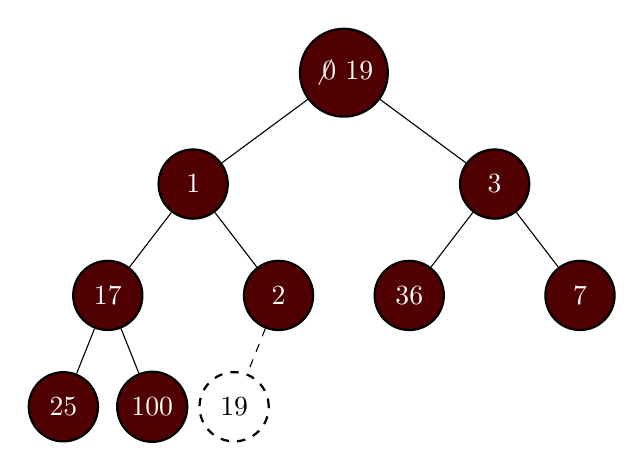
\begin{tikzpicture}
      \node[state] (0) {$\not 0$ 19};
      \node[state, below left of=0, xshift=-0.5cm] (1) {1};
      \node[state, below right of=0, xshift=0.5cm] (3) {3};
      \node[state, below left of=1, xshift=0.33cm] (17) {17};
      \node[state, below right of=1, xshift=-0.33cm] (2) {2};
      \node[state, below left of=3, xshift=0.33cm] (36) {36};
      \node[state, below right of=3, xshift=-0.33cm] (7) {7};
      \node[state, below left of=17, xshift=0.85cm] (25) {25};
      \node[state, below right of=17, xshift=-0.85cm] (100) {100};
      \node[selected, dashed, below left of=2, xshift=0.85cm] (19) {19};

      \draw (0) edge node{} (1)
      (0) edge node{} (3)
      (1) edge node{} (17)
      (1) edge node{} (2)
      (3) edge node{} (36)
      (3) edge node{} (7)
      (17) edge node{} (25)
      (17) edge node{} (100)
      (2) edge[dashed] node{} (19);
    \end{tikzpicture}
    \caption{Copy `19' into `0' and erase the last node}
    \label{fig:begin_remove}
  \end{figure}
\end{frame}

\begin{frame}{Removal}
  \begin{figure}[ht] % ’ht’ tells LaTeX to place the figure ’here’ or at the top of the page
    \centering % centers the figure
    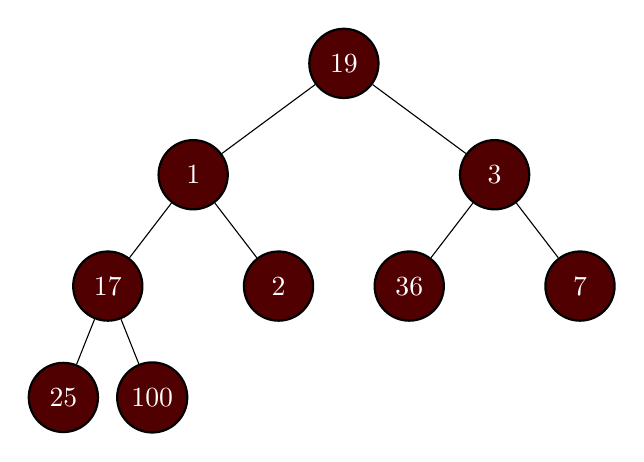
\begin{tikzpicture}
      \node[state] (0) {19};
      \node[state, below left of=0, xshift=-0.5cm] (1) {1};
      \node[state, below right of=0, xshift=0.5cm] (3) {3};
      \node[state, below left of=1, xshift=0.33cm] (17) {17};
      \node[state, below right of=1, xshift=-0.33cm] (2) {2};
      \node[state, below left of=3, xshift=0.33cm] (36) {36};
      \node[state, below right of=3, xshift=-0.33cm] (7) {7};
      \node[state, below left of=17, xshift=0.85cm] (25) {25};
      \node[state, below right of=17, xshift=-0.85cm] (100) {100};

      \draw (0) edge node{} (1)
      (0) edge node{} (3)
      (1) edge node{} (17)
      (1) edge node{} (2)
      (3) edge node{} (36)
      (3) edge node{} (7)
      (17) edge node{} (25)
      (17) edge node{} (100);
    \end{tikzpicture}
    \caption{After deleting last node}
    \label{fig:after_del_last_node}
  \end{figure}
  The root is now out of order, so we need to perform a similar operation to Upheap. We call this operation Downheap.
\end{frame}

\subsubsection{Downheap}

\begin{frame}{Downheap}
  Compare the root with its children and swap with the most \emph{extreme} child. For a min-heap, this is the smallest child.
  \begin{figure}[ht] % ’ht’ tells LaTeX to place the figure ’here’ or at the top of the page
    \centering % centers the figure
    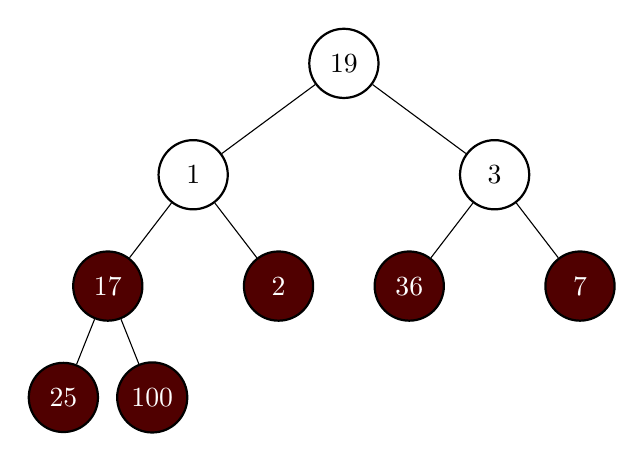
\begin{tikzpicture}
      \node[selected] (0) {19};
      \node[selected, below left of=0, xshift=-0.5cm] (1) {1};
      \node[selected, below right of=0, xshift=0.5cm] (3) {3};
      \node[state, below left of=1, xshift=0.33cm] (17) {17};
      \node[state, below right of=1, xshift=-0.33cm] (2) {2};
      \node[state, below left of=3, xshift=0.33cm] (36) {36};
      \node[state, below right of=3, xshift=-0.33cm] (7) {7};
      \node[state, below left of=17, xshift=0.85cm] (25) {25};
      \node[state, below right of=17, xshift=-0.85cm] (100) {100};

      \draw (0) edge node{} (1)
      (0) edge node{} (3)
      (1) edge node{} (17)
      (1) edge node{} (2)
      (3) edge node{} (36)
      (3) edge node{} (7)
      (17) edge node{} (25)
      (17) edge node{} (100);
    \end{tikzpicture}
    \caption{Comparing 19 with its children}
    \label{fig:comp_19_1_3}
  \end{figure}
\end{frame}

\begin{frame}{Downheap}
  Swap `1' with `19' to correct the order. Because `1' was the smaller child, it is guaranteed to be in order with respect to `3', so we can continue downwards.
  \begin{figure}[ht] % ’ht’ tells LaTeX to place the figure ’here’ or at the top of the page
    \centering % centers the figure
    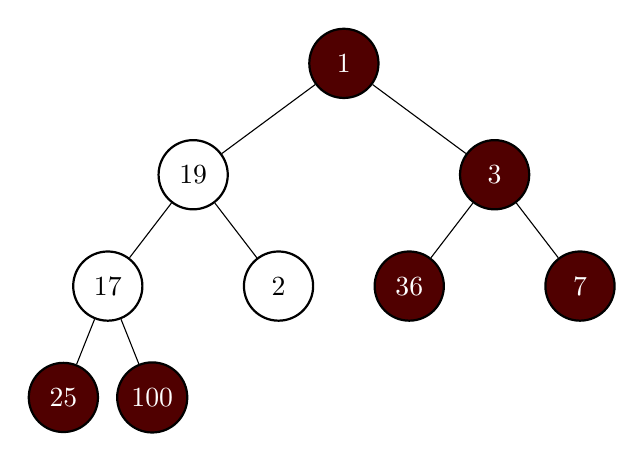
\begin{tikzpicture}
      \node[state] (0) {1};
      \node[selected, below left of=0, xshift=-0.5cm] (1) {19};
      \node[state, below right of=0, xshift=0.5cm] (3) {3};
      \node[selected, below left of=1, xshift=0.33cm] (17) {17};
      \node[selected, below right of=1, xshift=-0.33cm] (2) {2};
      \node[state, below left of=3, xshift=0.33cm] (36) {36};
      \node[state, below right of=3, xshift=-0.33cm] (7) {7};
      \node[state, below left of=17, xshift=0.85cm] (25) {25};
      \node[state, below right of=17, xshift=-0.85cm] (100) {100};

      \draw (0) edge node{} (1)
      (0) edge node{} (3)
      (1) edge node{} (17)
      (1) edge node{} (2)
      (3) edge node{} (36)
      (3) edge node{} (7)
      (17) edge node{} (25)
      (17) edge node{} (100);
    \end{tikzpicture}
    \caption{Comparing 19 with its children}
    \label{fig:comp_19_17_2}
  \end{figure}
\end{frame}

\begin{frame}{Downheap}
  Swap `2' with `19' to correct the order. As `19' is now a leaf, we can stop. If the node is ever in the correct order before becoming a leaf, we can stop then too.
  \begin{figure}[ht] % ’ht’ tells LaTeX to place the figure ’here’ or at the top of the page
    \centering % centers the figure
    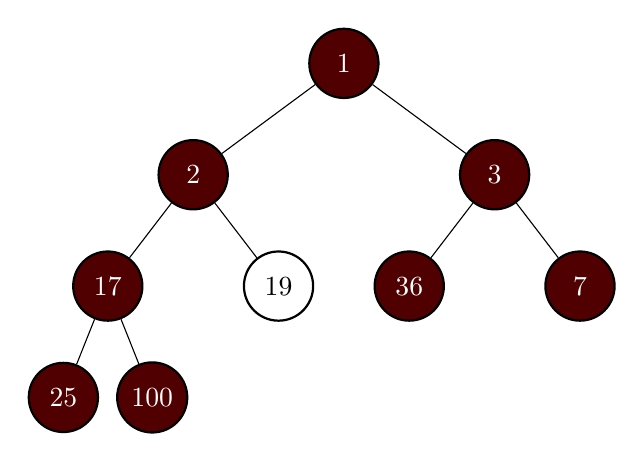
\begin{tikzpicture}
      \node[state] (0) {1};
      \node[state, below left of=0, xshift=-0.5cm] (1) {2};
      \node[state, below right of=0, xshift=0.5cm] (3) {3};
      \node[state, below left of=1, xshift=0.33cm] (17) {17};
      \node[selected, below right of=1, xshift=-0.33cm] (2) {19};
      \node[state, below left of=3, xshift=0.33cm] (36) {36};
      \node[state, below right of=3, xshift=-0.33cm] (7) {7};
      \node[state, below left of=17, xshift=0.85cm] (25) {25};
      \node[state, below right of=17, xshift=-0.85cm] (100) {100};

      \draw (0) edge node{} (1)
      (0) edge node{} (3)
      (1) edge node{} (17)
      (1) edge node{} (2)
      (3) edge node{} (36)
      (3) edge node{} (7)
      (17) edge node{} (25)
      (17) edge node{} (100);
    \end{tikzpicture}
    \caption{19 is now a leaf}
    \label{fig:comp_19_leaf}
  \end{figure}
\end{frame}

\begin{frame}{Downheap}
  \begin{figure}[ht] % ’ht’ tells LaTeX to place the figure ’here’ or at the top of the page
    \centering % centers the figure
    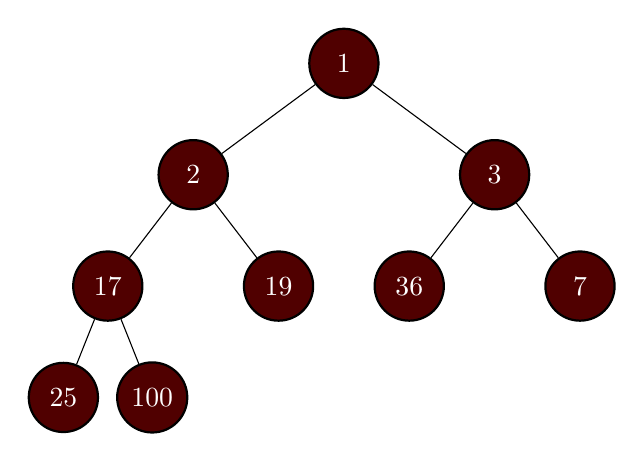
\begin{tikzpicture}
      \node[state] (0) {1};
      \node[state, below left of=0, xshift=-0.5cm] (1) {2};
      \node[state, below right of=0, xshift=0.5cm] (3) {3};
      \node[state, below left of=1, xshift=0.33cm] (17) {17};
      \node[state, below right of=1, xshift=-0.33cm] (2) {19};
      \node[state, below left of=3, xshift=0.33cm] (36) {36};
      \node[state, below right of=3, xshift=-0.33cm] (7) {7};
      \node[state, below left of=17, xshift=0.85cm] (25) {25};
      \node[state, below right of=17, xshift=-0.85cm] (100) {100};

      \draw (0) edge node{} (1)
      (0) edge node{} (3)
      (1) edge node{} (17)
      (1) edge node{} (2)
      (3) edge node{} (36)
      (3) edge node{} (7)
      (17) edge node{} (25)
      (17) edge node{} (100);
    \end{tikzpicture}
    \caption{After removing the root from the heap}
    \label{fig:after_removal}
  \end{figure}
\end{frame}

\subsubsection{Summary}

\begin{frame}{Removal Summary}
  \begin{algorithm}[H]
    \caption{Remove with Included Downheap}\label{alg:heap_remove}
    \begin{algorithmic}
      \Require $T$ is a binary min-heap
      \State $T$.\texttt{root}.\texttt{value} $\gets$ $T$.\texttt{get\_last}$()$.\texttt{value}  \Comment{Copy last into root}
      \State $i \gets T$.\texttt{get\_node}$(T\text{.}\texttt{root})$  \Comment{$i$ refers to root}
      \While{$i$ \textbf{is not} \textit{leaf} \textbf{and} ($i\text{.}\texttt{value} > i\text{.}\texttt{left\_child}\text{.}\texttt{value}$ \textbf{or} $i\text{.}\texttt{value} > i\text{.}\texttt{right\_child}\text{.}\texttt{value}$)}
      \State $\texttt{min\_child}\gets$ child of $i$ with minimum value
      \State \textbf{swap}$(i,\ \texttt{min\_child})$ \Comment{Downheap root}
      \EndWhile
    \end{algorithmic}
  \end{algorithm}
  This algorithm assumes that if $i$.\texttt{right\_child} does not exist, its value is $\infty$. Therefore, it cannot be the \texttt{min\_child}.
\end{frame}

\subsubsection{Arbitrary Removal}
\begin{frame}{Arbitrary Removal}
  \textbf{You do not need to know this.} That said, the process is similar. We take in the node we wish to remove and copy the last node into it. Then we perform Downheap from that node until it terminates. This task becomes difficult if we are asked to find the node we wish to remove. Searching in a Binary Heap is a painful experience, as you'll soon see in the next section.
\end{frame}

\subsection{Search}

\begin{frame}{Search}
  \begin{itemize}
    \item Binary Heaps are not Binary Search Trees
    \item The search performance is really bad $O(n)$
          \begin{itemize}
            \item This is \emph{despite} the ordering property.
          \end{itemize}
    \item So why use heaps?
          \begin{itemize}
            \item Getting minimum (or maximum for max-heaps) is $O(1)$
            \item Removing minimum (or maximum) is $O(\log n)$
            \item Inserting is $O(\log n)$
            \item Constructing a Heap from Scratch (Heapify/Bottom Up) is $O(n)$
          \end{itemize}
    \item Heaps are only bad at search, so use a Search Tree for that!
    \item Heaps are great for Priority Queues and other Priority Systems.
  \end{itemize}
\end{frame}

\begin{frame}{Search}
  Search can be done
  \begin{itemize}
    \item linearly on the array (if array representation) or
    \item through a tree traversal (if tree representation).
  \end{itemize}
  Either approach yields $O(n)$ time, so we are stuck.
\end{frame}

\subsection{Heapify}

\begin{frame}{Heapify a.k.a. Bottom-Up Heap Construction}
  \begin{itemize}
    \item Given an array of values, we need to convert it into a Heap.
          \begin{itemize}
            \item Well, structurally, it is already a heap because all heaps are Arrays.
            \item Therefore, we have to rearrange the data in the array.
          \end{itemize}
    \item We have discussed Sorting before, which is an $O(n\log n)$ problem in the best of times for a Comparison-based sorting algorithm.
          \begin{itemize}
            \item Thankfully, Heapify is not exactly sorting though it does make the array somewhat more sorted.
          \end{itemize}
    \item Because Heapify does not require thoroughly sorting the array, it has a better Big-O bound of $O(n)$.
          \begin{itemize}
            \item Thus, this process improves upon blindly calling Heap Insert for the $n$ elements, which is $O(n\log n)$.
          \end{itemize}
    \item We can use Heapify and Remove to sort data. We call this, Heapsort $O(n\log n)$.
  \end{itemize}
\end{frame}

\begin{frame}{Heapify}
  \begin{algorithm}[H]
    \caption{Bottom Up Heap Construction}\label{alg:heapify}
    \begin{algorithmic}
      \Require $V$ is a \texttt{vector}
      \For{$i\gets V\text{.}\texttt{size}() / 2 - 1$ \textbf{to} 0} \Comment{\emph{includes} 0}
      \State \texttt{Downheap}$(i)$ \Comment{perform the Downheap loop on $i$}
      \EndFor
    \end{algorithmic}
  \end{algorithm}
  This assumes that you took the loop from \texttt{remove} and made it into a \texttt{Downheap} function, which is probably a \emph{good} idea to do anyway.

  The following algorithm is recursive and can better illustrate what is happening. It is a bit less efficient, though, so the above algorithm is good to use.
\end{frame}

\begin{frame}{Heapify}
  \begin{algorithm}[H]
    \caption{Bottom Up Heap Construction}\label{alg:heapify_2}
    \begin{algorithmic}
      \Require $L$ is a \texttt{list} (or other linked list), though a vector works too
      \If{$L$.\texttt{empty}$()$}
      \State \Return an empty heap
      \EndIf
      \State $e\gets L$.\texttt{front}$()$
      \State $L$.\texttt{pop\_front}$()$
      \State Split $L$ into two lists, $L_1$ and $L_2$, each of size $(n-1)/2$
      \State $T_1\gets\texttt{Heapify}(L_1)$
      \State $T_2\gets\texttt{Heapify}(L_2)$
      \State Create binary tree $T$ with root $r$ storing $e$, left subtree $T_1$, and right subtree $T_2$
      \State Perform a down-heap bubbling from the root $r$ of $T$, if necessary
    \end{algorithmic}
  \end{algorithm}
  From: \textit{Data Structures \& Algorithms} by Goodrich et al.
\end{frame}

\begin{frame}{Heapify}
  We now perform Heapify on the following data:

  \begin{tabular}{c|c}
    Array Index & Array Value \\\hline
    0           & 14          \\
    1           & 9           \\
    2           & 25          \\
    3           & 16          \\
    4           & 15          \\
    5           & 5           \\
    6           & 4           \\
    7           & 12          \\
    8           & 8           \\
    9           & 11          \\
    10          & 6           \\
    11          & 7           \\
    12          & 27          \\
    13          & 23          \\
    14          & 20
  \end{tabular}
\end{frame}

\begin{frame}{Heapify}
  \begin{figure}[ht] % ’ht’ tells LaTeX to place the figure ’here’ or at the top of the page
    \centering % centers the figure
    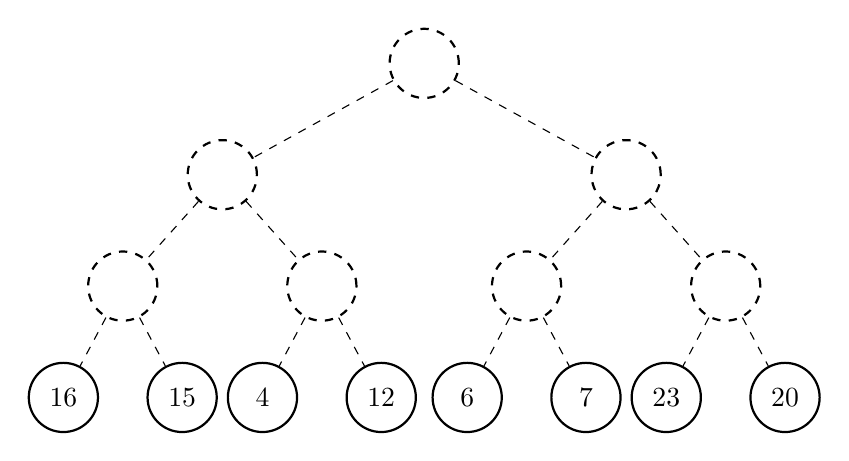
\begin{tikzpicture}
      \node[state, dashed, fill=none] (4) {};
      \node[state, dashed, fill=none, below left of=4, xshift=-1.15cm] (5) {};
      \node[state, dashed, fill=none, below right of=4, xshift=1.15cm] (6) {};
      \node[state, dashed, fill=none, below left of=5, xshift=0.15cm] (15) {};
      \node[state, dashed, fill=none, below right of=5, xshift=-0.15cm] (9) {};
      \node[state, dashed, fill=none, below left of=6, xshift=0.15cm] (7) {};
      \node[state, dashed, fill=none, below right of=6, xshift=-0.15cm] (20) {};
      \node[selected, below left of=15, xshift=0.66cm] (16) {16};
      \node[selected, below right of=15, xshift=-0.66cm] (25) {15};
      \node[selected, below left of=9, xshift=0.66cm] (14) {4};
      \node[selected, below right of=9, xshift=-0.66cm] (12) {12};
      \node[selected, below left of=7, xshift=0.66cm] (11) {6};
      \node[selected, below right of=7, xshift=-0.66cm] (8) {7};
      \node[selected, below left of=20, xshift=0.66cm] (23) {23};
      \node[selected, below right of=20, xshift=-0.66cm] (27) {20};

      \draw (4) edge[dashed] node{} (5)
      (4) edge[dashed] node{} (6)
      (5) edge[dashed] node{} (15)
      (5) edge[dashed] node{} (9)
      (6) edge[dashed] node{} (7)
      (6) edge[dashed] node{} (20)
      (15) edge[dashed] node{} (16)
      (15) edge[dashed] node{} (25)
      (9) edge[dashed] node{} (14)
      (9) edge[dashed] node{} (12)
      (7) edge[dashed] node{} (11)
      (7) edge[dashed] node{} (8)
      (20) edge[dashed] node{} (23)
      (20) edge[dashed] node{} (27);
    \end{tikzpicture}
    \caption{Construct trivial heaps}
    \label{fig:heapify_step_1}
  \end{figure}
\end{frame}

\begin{frame}{Heapify}
  \begin{figure}[ht] % ’ht’ tells LaTeX to place the figure ’here’ or at the top of the page
    \centering % centers the figure
    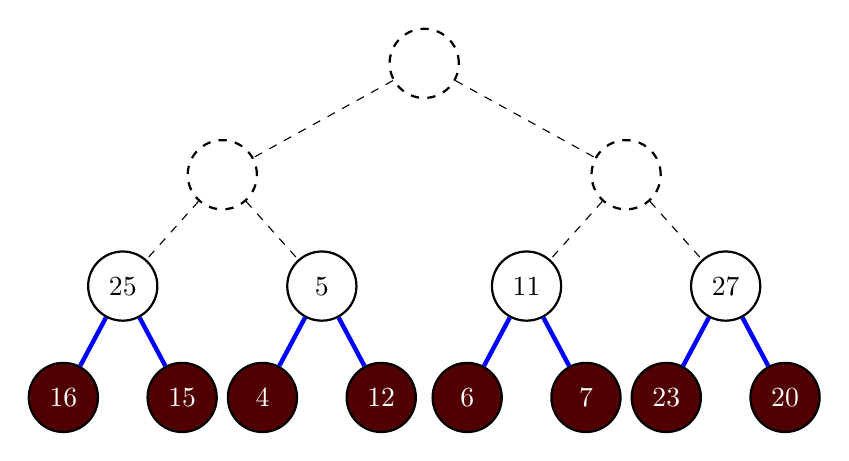
\begin{tikzpicture}
      \node[state, dashed, fill=none] (4) {};
      \node[state, dashed, fill=none, below left of=4, xshift=-1.15cm] (5) {};
      \node[state, dashed, fill=none, below right of=4, xshift=1.15cm] (6) {};
      \node[selected, below left of=5, xshift=0.15cm] (15) {25};
      \node[selected, below right of=5, xshift=-0.15cm] (9) {5};
      \node[selected, below left of=6, xshift=0.15cm] (7) {11};
      \node[selected, below right of=6, xshift=-0.15cm] (20) {27};
      \node[state, below left of=15, xshift=0.66cm] (16) {16};
      \node[state, below right of=15, xshift=-0.66cm] (25) {15};
      \node[state, below left of=9, xshift=0.66cm] (14) {4};
      \node[state, below right of=9, xshift=-0.66cm] (12) {12};
      \node[state, below left of=7, xshift=0.66cm] (11) {6};
      \node[state, below right of=7, xshift=-0.66cm] (8) {7};
      \node[state, below left of=20, xshift=0.66cm] (23) {23};
      \node[state, below right of=20, xshift=-0.66cm] (27) {20};

      \draw (4) edge[dashed] node{} (5)
      (4) edge[dashed] node{} (6)
      (5) edge[dashed] node{} (15)
      (5) edge[dashed] node{} (9)
      (6) edge[dashed] node{} (7)
      (6) edge[dashed] node{} (20)
      (15) edge[ultra thick, draw=blue] node{} (16)
      (15) edge[ultra thick, draw=blue] node{} (25)
      (9) edge[ultra thick, draw=blue] node{} (14)
      (9) edge[ultra thick, draw=blue] node{} (12)
      (7) edge[ultra thick, draw=blue] node{} (11)
      (7) edge[ultra thick, draw=blue] node{} (8)
      (20) edge[ultra thick, draw=blue] node{} (23)
      (20) edge[ultra thick, draw=blue] node{} (27);
    \end{tikzpicture}
    \caption{Insert third node}
    \label{fig:heapify_step_2}
  \end{figure}
\end{frame}

\begin{frame}{Heapify}
  \begin{figure}[ht] % ’ht’ tells LaTeX to place the figure ’here’ or at the top of the page
    \centering % centers the figure
    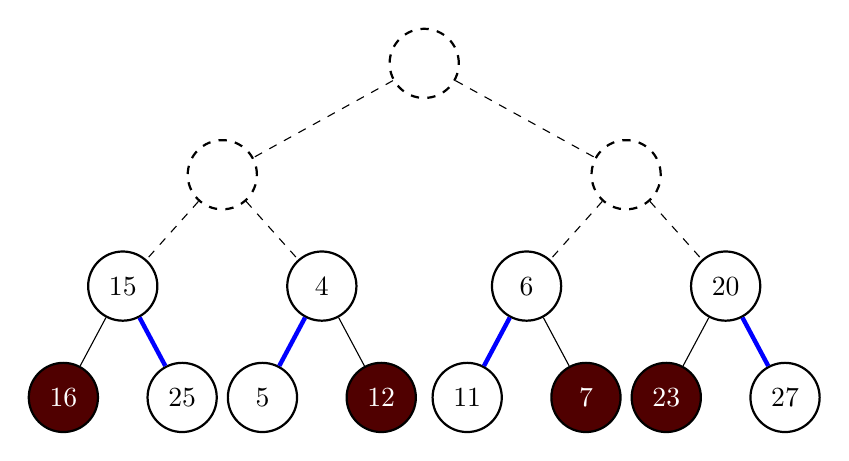
\begin{tikzpicture}
      \node[state, dashed, fill=none] (4) {};
      \node[state, dashed, fill=none, below left of=4, xshift=-1.15cm] (5) {};
      \node[state, dashed, fill=none, below right of=4, xshift=1.15cm] (6) {};
      \node[selected, below left of=5, xshift=0.15cm] (15) {15};
      \node[selected, below right of=5, xshift=-0.15cm] (9) {4};
      \node[selected, below left of=6, xshift=0.15cm] (7) {6};
      \node[selected, below right of=6, xshift=-0.15cm] (20) {20};
      \node[state, below left of=15, xshift=0.66cm] (16) {16};
      \node[selected, below right of=15, xshift=-0.66cm] (25) {25};
      \node[selected, below left of=9, xshift=0.66cm] (14) {5};
      \node[state, below right of=9, xshift=-0.66cm] (12) {12};
      \node[selected, below left of=7, xshift=0.66cm] (11) {11};
      \node[state, below right of=7, xshift=-0.66cm] (8) {7};
      \node[state, below left of=20, xshift=0.66cm] (23) {23};
      \node[selected, below right of=20, xshift=-0.66cm] (27) {27};

      \draw (4) edge[dashed] node{} (5)
      (4) edge[dashed] node{} (6)
      (5) edge[dashed] node{} (15)
      (5) edge[dashed] node{} (9)
      (6) edge[dashed] node{} (7)
      (6) edge[dashed] node{} (20)
      (15) edge node{} (16)
      (15) edge[ultra thick, draw=blue] node{} (25)
      (9) edge[ultra thick, draw=blue] node{} (14)
      (9) edge node{} (12)
      (7) edge[ultra thick, draw=blue] node{} (11)
      (7) edge node{} (8)
      (20) edge node{} (23)
      (20) edge[ultra thick, draw=blue] node{} (27);
    \end{tikzpicture}
    \caption{Downheap as necessary}
    \label{fig:heapify_step_3}
  \end{figure}
\end{frame}

\begin{frame}{Heapify}
  \begin{figure}[ht] % ’ht’ tells LaTeX to place the figure ’here’ or at the top of the page
    \centering % centers the figure
    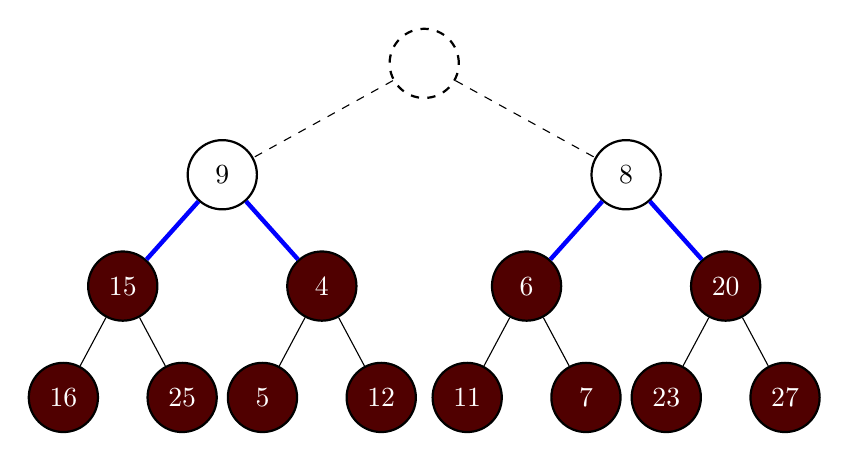
\begin{tikzpicture}
      \node[state, dashed, fill=none] (4) {};
      \node[selected, below left of=4, xshift=-1.15cm] (5) {9};
      \node[selected, below right of=4, xshift=1.15cm] (6) {8};
      \node[state, below left of=5, xshift=0.15cm] (15) {15};
      \node[state, below right of=5, xshift=-0.15cm] (9) {4};
      \node[state, below left of=6, xshift=0.15cm] (7) {6};
      \node[state, below right of=6, xshift=-0.15cm] (20) {20};
      \node[state, below left of=15, xshift=0.66cm] (16) {16};
      \node[state, below right of=15, xshift=-0.66cm] (25) {25};
      \node[state, below left of=9, xshift=0.66cm] (14) {5};
      \node[state, below right of=9, xshift=-0.66cm] (12) {12};
      \node[state, below left of=7, xshift=0.66cm] (11) {11};
      \node[state, below right of=7, xshift=-0.66cm] (8) {7};
      \node[state, below left of=20, xshift=0.66cm] (23) {23};
      \node[state, below right of=20, xshift=-0.66cm] (27) {27};

      \draw (4) edge[dashed] node{} (5)
      (4) edge[dashed] node{} (6)
      (5) edge[ultra thick, draw=blue] node{} (15)
      (5) edge[ultra thick, draw=blue] node{} (9)
      (6) edge[ultra thick, draw=blue] node{} (7)
      (6) edge[ultra thick, draw=blue] node{} (20)
      (15) edge node{} (16)
      (15) edge node{} (25)
      (9) edge node{} (14)
      (9) edge node{} (12)
      (7) edge node{} (11)
      (7) edge node{} (8)
      (20) edge node{} (23)
      (20) edge node{} (27);
    \end{tikzpicture}
    \caption{Combine heaps into bigger heaps adding root}
    \label{fig:heapify_step_4}
  \end{figure}
\end{frame}

\begin{frame}{Heapify}
  \begin{figure}[ht] % ’ht’ tells LaTeX to place the figure ’here’ or at the top of the page
    \centering % centers the figure
    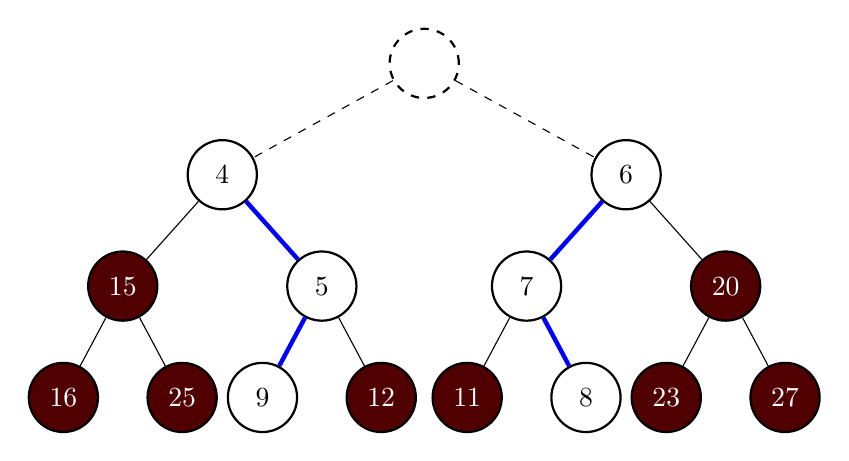
\begin{tikzpicture}
      \node[state, dashed, fill=none] (4) {};
      \node[selected, below left of=4, xshift=-1.15cm] (5) {4};
      \node[selected, below right of=4, xshift=1.15cm] (6) {6};
      \node[state, below left of=5, xshift=0.15cm] (15) {15};
      \node[selected, below right of=5, xshift=-0.15cm] (9) {5};
      \node[selected, below left of=6, xshift=0.15cm] (7) {7};
      \node[state, below right of=6, xshift=-0.15cm] (20) {20};
      \node[state, below left of=15, xshift=0.66cm] (16) {16};
      \node[state, below right of=15, xshift=-0.66cm] (25) {25};
      \node[selected, below left of=9, xshift=0.66cm] (14) {9};
      \node[state, below right of=9, xshift=-0.66cm] (12) {12};
      \node[state, below left of=7, xshift=0.66cm] (11) {11};
      \node[selected, below right of=7, xshift=-0.66cm] (8) {8};
      \node[state, below left of=20, xshift=0.66cm] (23) {23};
      \node[state, below right of=20, xshift=-0.66cm] (27) {27};

      \draw (4) edge[dashed] node{} (5)
      (4) edge[dashed] node{} (6)
      (5) edge node{} (15)
      (5) edge[ultra thick, draw=blue] node{} (9)
      (6) edge[ultra thick, draw=blue] node{} (7)
      (6) edge node{} (20)
      (15) edge node{} (16)
      (15) edge node{} (25)
      (9) edge[ultra thick, draw=blue] node{} (14)
      (9) edge node{} (12)
      (7) edge node{} (11)
      (7) edge[ultra thick, draw=blue] node{} (8)
      (20) edge node{} (23)
      (20) edge node{} (27);
    \end{tikzpicture}
    \caption{Downheap as necessary}
    \label{fig:heapify_step_5}
  \end{figure}
\end{frame}

\begin{frame}{Heapify}
  \begin{figure}[ht] % ’ht’ tells LaTeX to place the figure ’here’ or at the top of the page
    \centering % centers the figure
    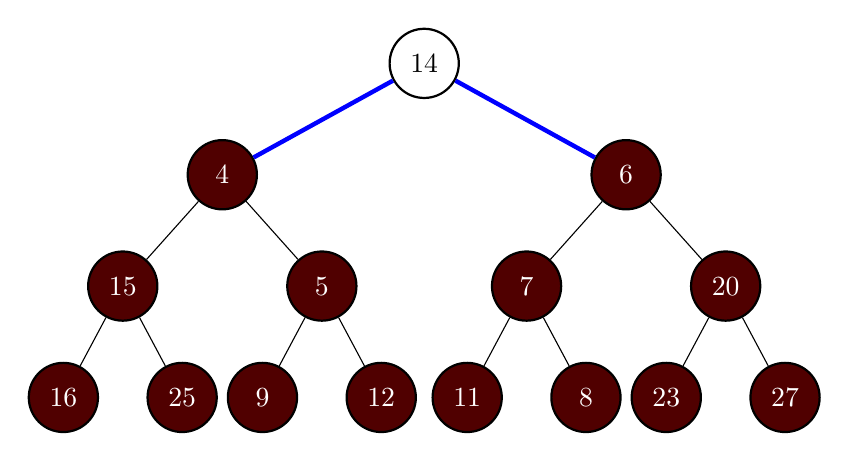
\begin{tikzpicture}
      \node[selected, fill=none] (4) {14};
      \node[state, below left of=4, xshift=-1.15cm] (5) {4};
      \node[state, below right of=4, xshift=1.15cm] (6) {6};
      \node[state, below left of=5, xshift=0.15cm] (15) {15};
      \node[state, below right of=5, xshift=-0.15cm] (9) {5};
      \node[state, below left of=6, xshift=0.15cm] (7) {7};
      \node[state, below right of=6, xshift=-0.15cm] (20) {20};
      \node[state, below left of=15, xshift=0.66cm] (16) {16};
      \node[state, below right of=15, xshift=-0.66cm] (25) {25};
      \node[state, below left of=9, xshift=0.66cm] (14) {9};
      \node[state, below right of=9, xshift=-0.66cm] (12) {12};
      \node[state, below left of=7, xshift=0.66cm] (11) {11};
      \node[state, below right of=7, xshift=-0.66cm] (8) {8};
      \node[state, below left of=20, xshift=0.66cm] (23) {23};
      \node[state, below right of=20, xshift=-0.66cm] (27) {27};

      \draw (4) edge[ultra thick, draw=blue] node{} (5)
      (4) edge[ultra thick, draw=blue] node{} (6)
      (5) edge node{} (15)
      (5) edge node{} (9)
      (6) edge node{} (7)
      (6) edge node{} (20)
      (15) edge node{} (16)
      (15) edge node{} (25)
      (9) edge node{} (14)
      (9) edge node{} (12)
      (7) edge node{} (11)
      (7) edge node{} (8)
      (20) edge node{} (23)
      (20) edge node{} (27);
    \end{tikzpicture}
    \caption{Insert final root}
    \label{fig:heapify_step_6}
  \end{figure}
\end{frame}

\begin{frame}{Heapify}
  \begin{figure}[ht] % ’ht’ tells LaTeX to place the figure ’here’ or at the top of the page
    \centering % centers the figure
    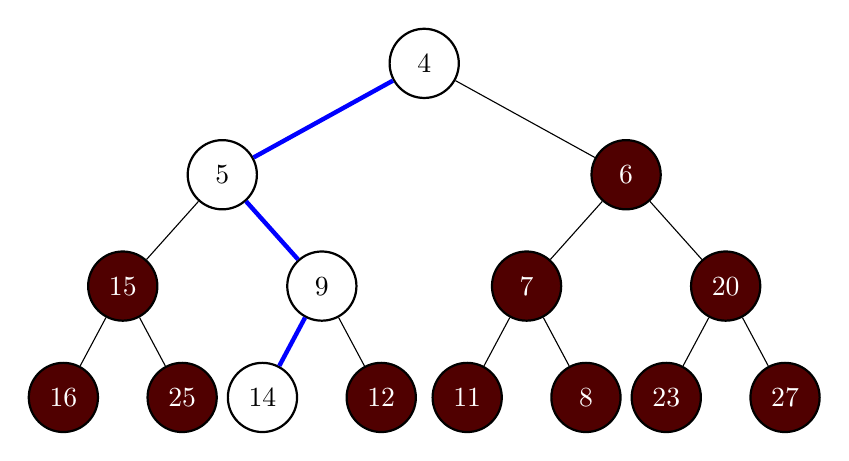
\begin{tikzpicture}
      \node[selected, fill=none] (4) {4};
      \node[selected, below left of=4, xshift=-1.15cm] (5) {5};
      \node[state, below right of=4, xshift=1.15cm] (6) {6};
      \node[state, below left of=5, xshift=0.15cm] (15) {15};
      \node[selected, below right of=5, xshift=-0.15cm] (9) {9};
      \node[state, below left of=6, xshift=0.15cm] (7) {7};
      \node[state, below right of=6, xshift=-0.15cm] (20) {20};
      \node[state, below left of=15, xshift=0.66cm] (16) {16};
      \node[state, below right of=15, xshift=-0.66cm] (25) {25};
      \node[selected, below left of=9, xshift=0.66cm] (14) {14};
      \node[state, below right of=9, xshift=-0.66cm] (12) {12};
      \node[state, below left of=7, xshift=0.66cm] (11) {11};
      \node[state, below right of=7, xshift=-0.66cm] (8) {8};
      \node[state, below left of=20, xshift=0.66cm] (23) {23};
      \node[state, below right of=20, xshift=-0.66cm] (27) {27};

      \draw (4) edge[ultra thick, draw=blue] node{} (5)
      (4) edge node{} (6)
      (5) edge node{} (15)
      (5) edge[ultra thick, draw=blue] node{} (9)
      (6) edge node{} (7)
      (6) edge node{} (20)
      (15) edge node{} (16)
      (15) edge node{} (25)
      (9) edge[ultra thick, draw=blue] node{} (14)
      (9) edge node{} (12)
      (7) edge node{} (11)
      (7) edge node{} (8)
      (20) edge node{} (23)
      (20) edge node{} (27);
    \end{tikzpicture}
    \caption{Downheap as necessary}
    \label{fig:heapify_step_7}
  \end{figure}
\end{frame}

\begin{frame}{Heapify}
  The final Heap Array:

  \begin{tabular}{c|c|c}
    Array Index & Array Value (originally) & Heap Value \\\hline
    0           & 14                       & 4          \\
    1           & 9                        & 5          \\
    2           & 25                       & 6          \\
    3           & 16                       & 15         \\
    4           & 15                       & 9          \\
    5           & 5                        & 7          \\
    6           & 4                        & 20         \\
    7           & 12                       & 16         \\
    8           & 8                        & 25         \\
    9           & 11                       & 14         \\
    10          & 6                        & 12         \\
    11          & 7                        & 11         \\
    12          & 27                       & 8          \\
    13          & 23                       & 23         \\
    14          & 20                       & 27
  \end{tabular}
\end{frame}

\subsection{Heap Sort}

\begin{frame}{Heap Sort}
  \begin{algorithm}[H]
    \caption{Heap Sort}\label{alg:heap_sort}
    \begin{algorithmic}
      \Require $V$ is a container (\texttt{vector} or \texttt{list})
      \State $S\gets\{\}$ \Comment{$S$ is the return vector which will be sorted}
      \State \texttt{Heapify}$(V)$ \Comment{Reorder $V$ to heap ordering $O(n)$}
      \While{$V$ \textbf{is not} \texttt{empty}} \Comment{loops $n$ times}
      \State $S$.\texttt{push\_back}$(V\text{.}\texttt{remove\_min}())$ \Comment{Heap remove min $O(\log n)$}
      \EndWhile
    \end{algorithmic}
  \end{algorithm}
  So the function is $f(n)=O(n)+n\cdot O(\log n)=O(n) + O(n\log n)=O(n\log n)$.
\end{frame}

\section{Conclusion}

\subsection{Conclusion}

\begin{frame}{Conclusion}
  \begin{itemize}
    \item Binary Heaps are useful for Priority Queues
    \item Don't search in Binary Heaps (unless you have to)
    \item Heapify lets us construct faster than repeatedly inserting
    \item Heap Sort builds a heap and removes one by one to get sorted order
          \begin{itemize}
            \item No direct comparisons (heap does them)
            \item Not recursive, but $O(n\log n)$ which is very nice
            \item Can relatively quickly get subset of values in sorted order
          \end{itemize}
  \end{itemize}
\end{frame}



%------------------------------------------------

\subsection{References}

\begin{frame}
  \frametitle{References}
  \footnotesize{
    \begin{thebibliography}{99} % Beamer does not support BibTeX so references must be inserted manually as below
      \bibitem[Smith, 2012]{p1} Michael T. Goodrich, Roberto Tamassia, David Mount
      \newblock Data Structures \& Algorithms
      \newblock \emph{Second Edition} Chapter 8.
    \end{thebibliography}
  }
\end{frame}

%------------------------------------------------

\subsection{Thank You}

\begin{frame}{}
  \centering \Huge
  \emph{Thank You!}
\end{frame}

%----------------------------------------------------------------------------------------


\end{document}


\end{document}